\documentclass[11pt]{beamer}

\usepackage[utf8]{inputenc}
\usepackage[magyar]{babel}
\usepackage[T1]{fontenc}
\usepackage{lmodern}
\usepackage{zi4}
\usepackage{multirow}
\usepackage{listings}
\usepackage{ragged2e} % For \justifying command

\usetheme{Warsaw}

\renewcommand\UrlFont{\ttfamily\footnotesize}

% no navigation symbols
\setbeamertemplate{navigation symbols}{} 

% frame numbers
\expandafter\def\expandafter\insertshorttitle\expandafter{%
  \insertshorttitle\hfill%
  \insertframenumber\,/\,\inserttotalframenumber}

\author{Nagy András}
\title{Komponens-alapú UML modellek fordításának vizsgálata}
\date{2019. január}

\begin{document}

\begin{frame}
\titlepage
\end{frame}

\begin{frame}
	\frametitle{Komponens-alapú megközelítés röviden}
	
	\begin{itemize}
		\item Program szereplőinek izolációja.
		\item A szereplők függetlenek a környezettől.
		\item Egymással interfész-portokkal kommunikálnak az egyes szereplők
		\item Előnyei: független telepíthetőség, explicit interfész függőségek..
	\end{itemize}
\end{frame}

\begin{frame}[fragile]
	\frametitle{Program szöveges modellezése}
	
	\begin{itemize}
		\item \textit{txtUML} keretrendszerben írjuk le a komponens-alapú modellt, Java-szerű nyelven, mely végrehajtható.
		\item Lefordítható egy szabványos UML2 modellre.
		\item A cél a kompozit struktúrák és akciók megfelelő UML2-es szabványának megtalálása, melyből hatékony C++ kód generálása.
	\end{itemize}
	
\end{frame}


\begin{frame}[fragile]
	\frametitle{Példa egy konkrét kompozit struktúrára}	
	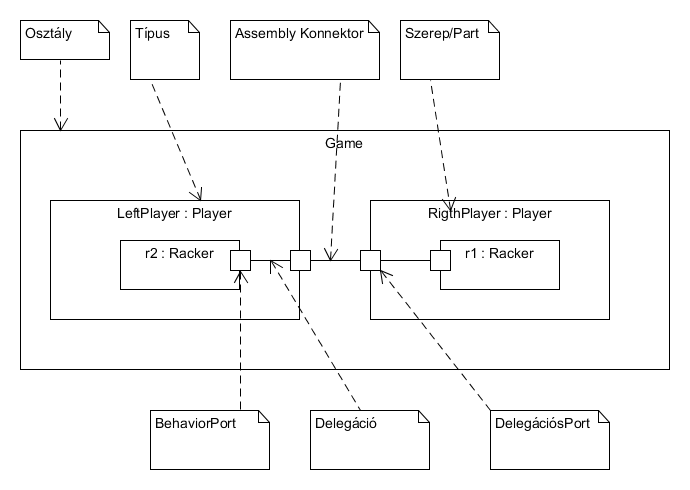
\includegraphics[scale=0.4]{vedes_demo.png}	
	Már az UML2-es reprezentáció sem triviális.

	
\end{frame}

\begin{frame}[fragile]	
	\frametitle{Főbb UML reprezentációs problémák}	
	\begin{itemize}
	\item Interfész port reprezentálása: mi a típusa, hogyan fejezzük ki az elvárt interfészt.
	\item Két port összekapcsolása futási időben.
	\item Porta való üzenetküldés.
	\item Mi a modell szemantikája??
	\end{itemize}
	
\end{frame}

\begin{frame}
	\frametitle{Példa: Konnektor, konnent UML-ben}
	\begin{itemize}
	\item A \textit{Connector} értelemszerű (de mi az a \textit{type} referencia?)
	\item A problémás a \textit{connect} művelet
		\begin{itemize}
		\item Nincs \textit{connect} akció UML-ben
		\item \textit{DefaultConstructionStrategy}  (de az a szerkezet nem mindig egyértelmű..)
		\item A \textit{CreateLinkAction} segítségével összeköthetünk két portot a konnektor típusa mentén (Itt jön be a \textit{type} referencia, mely egy asszociációnak felel, ezt még ki kell generálni.).
		\end{itemize}
	\end{itemize}
\end{frame}


\begin{frame}[fragile]	
	\frametitle{C++-ra való fordítása}	
	\begin{itemize}
	\item Sok alternatíva (típusbiztonság, adatreprezentációs különbségek, stb)
	\item Különböző elvárások a generált kóddal szemben (hatékonyság, olvashatóság, külső kóddal történő biztonságos illesztés, stb.)
	\item Ez főleg a megfelelő kertrendszerek kialakításából és az UML szemantika értelmezéséből áll.
	\item Ezeket a szempontokat figyelembe véve elemezni az egyes elemek generálását (interfész: 3+1, különböző port típusok: 2, konnektor struktúrák: 2,  kapcsolódási végpontok tárolása: 2 + 1,  portok összekapcsolásának kifejezése 2 + 1, üzenetküldés/fogadás: 2, üzenetfeldolgozás: 2).
	\end{itemize}
	
\end{frame}

\begin{frame}
	\frametitle{Üzenetáram eleje}
	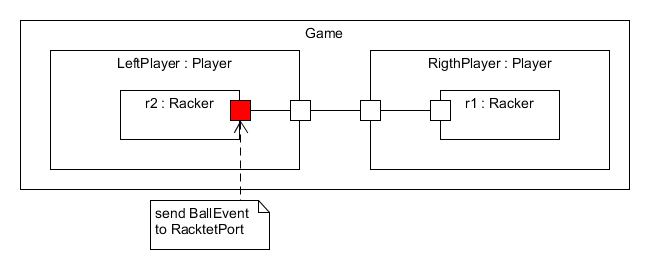
\includegraphics[scale=0.5]{vedes_demo_send.png}
	
	Kérdések:
	\begin{itemize}
	\item Hogyan reprezentáljuk a szabványban a portra való üzenetküldést, hogyan kell ezt értelmezni?
	\item Interfész portok reprezentálása, generálása?
	\end{itemize}
	
\end{frame}

\begin{frame}
	\frametitle{Portok naiv ábrázolása}
	\begin{center}
	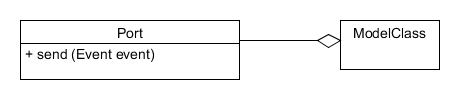
\includegraphics[scale=0.5]{vedes_demo_simple_send.png}
	\end{center}
	Problémák: 
	\begin{itemize}
	\item A port bármilyen üzenetet fogadhat, hol vannak az interfészek?
	\item Mi a send szemantikája, milyen UML akciónak felel meg?
	\end{itemize}


\end{frame}

\begin{frame}
	\frametitle{Interfész portok üzenetküldéssel}
	\begin{center}
	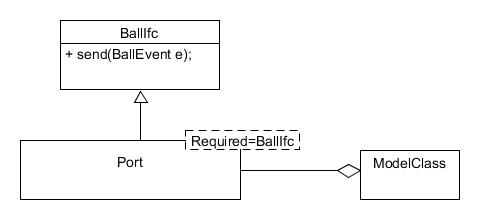
\includegraphics[scale=0.5]{vedes_demo_interface_send.png}
	\end{center}
	
	\begin{itemize}
	\item A típushelyességet biztosítottuk.
	\item A továbbiakban a \textit{send} szemantika érdekes.
	\end{itemize}

\end{frame}

\begin{frame}
	\frametitle{Üzenet továbbítása a szülő komponens felé - Delegáció}
	\begin{center}
	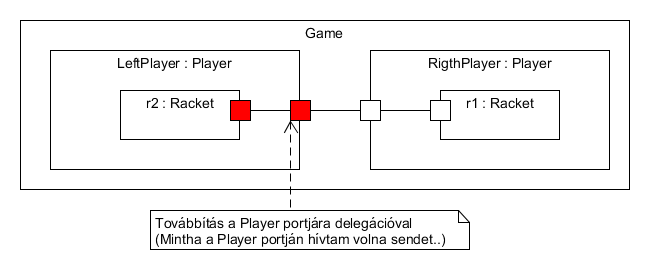
\includegraphics[scale=0.5]{vedes_demo_connect.png}
	\end{center}
	
	Problémák:
	\begin{itemize}
	\item Hogyan adom tovább az üzenet a szülő felé?
	\item Hogyan kapcsolom össze a gyerek és a szülő portját?
	\item Honnan tudom, hogy delegációs kapcsolat áll a két port között?
	\end{itemize}

\end{frame}


\begin{frame}
	\frametitle{Naiv kapcsolat referencia tárolás}
	\begin{center}
	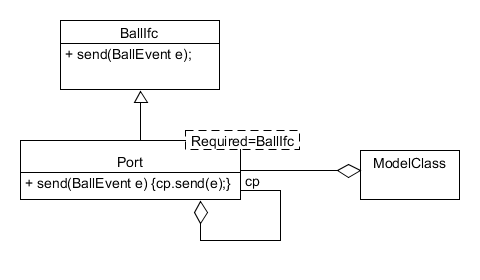
\includegraphics[scale=0.5]{vedes_demo_delegref.png}
	\end{center}
	Problémák:
	\begin{itemize}
	\item Delegációs kapcsolat esetén működik csak.
	\item Delegációs összekapcsolás esetén kell beállítani a referenciát.
	\end{itemize}

\end{frame}


\begin{frame}
	\frametitle{Üzenet átadása testvér komponensek - Assembly}
	\begin{center}
	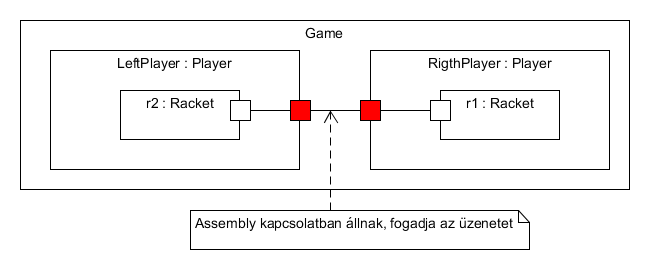
\includegraphics[scale=0.5]{vedes_demo_assconnect.png}
	\end{center}
	Újabb problémák:
	\begin{itemize}
	\item A \textit{send} másképp viselkedik, mint delegációs kapcsolat esetén.
	\item A jobb oldali célportnak nem delegálok, hanem fogadja az üzenetet, ami befele áramol tovább. (Az elvárt interfész érdekes számomra)
	\end{itemize}
		
\end{frame}

\begin{frame}
	\frametitle{Interfészek szétbontása}
	\begin{center}
	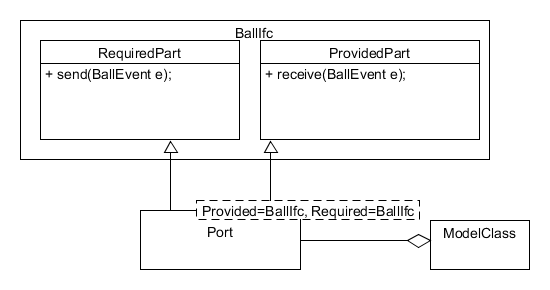
\includegraphics[scale=0.5]{vedes_demo_interface_send_rec.png}
	\end{center}
	\begin{itemize}
	\item Az PSCS szemantika szerint az üzenetküldés kontextusától függ az üzenetáram iránya.
	\item \textit{send} - belülről jött üzenetküldés, \textit{receive} - kívülről jött üzenet fogadása
	\end{itemize}
\end{frame}

\begin{frame}
	\frametitle{Kapcsolat referencia szétbontása}
	\begin{center}
	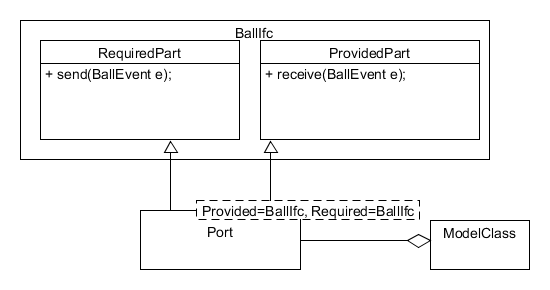
\includegraphics[scale=0.5]{vedes_demo_interface_send_rec.png}
	\end{center}
	\begin{itemize}
	\item A kapcsolat referenciát öröklődéssel tehetjük a legtisztábban poliformmá.
	\item Az assembly kapcsolódás miatt \textit{send} helyett \textit{receive}-et kell hívni a kapcsolt porton.
	\end{itemize}
\end{frame}


\begin{frame}
	\frametitle{Kapcsolat referencia szétbontása}
	\begin{center}
	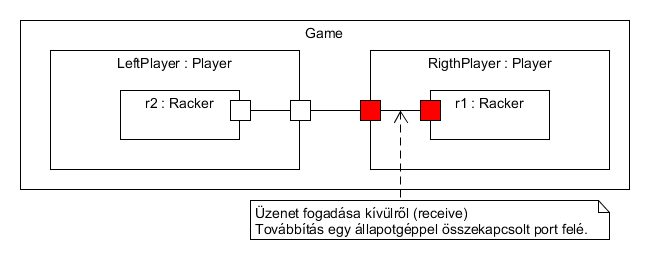
\includegraphics[scale=0.5]{vedes_demo_recived.png}
	\end{center}
	\begin{itemize}
	\item A delegáció miatt továbbítani kell az üzenetet a belső komponens felé.
	\item Ez a kapcsolat azonban különbözik az általános kapcsolat referenciától.
	\item Mintha a gyerek \textit{receive}-jét hívtuk volna..
	\end{itemize}
\end{frame}

\begin{frame}
	\frametitle{Gyerek felé továbbítás delegáció esetén}
	\begin{center}
	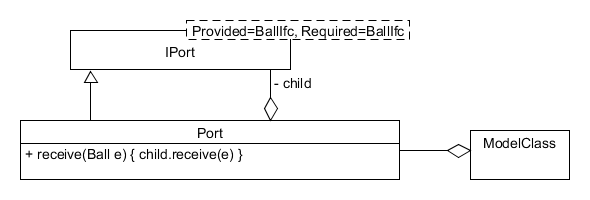
\includegraphics[scale=0.5]{vedes_demo_notbehav_port.png}
	\end{center}
	\begin{itemize}
	\item A gyerek referenciát egy delegációs összekapcsolás állítja be.
	\item Más lesz ennek a viselkedése állapotgéppel összekapcsolt port esetén, ezért kell az interfész..
	\end{itemize}
\end{frame}

\begin{frame}
	\frametitle{Gyerek felé továbbítás delegáció esetén}
	\begin{center}
	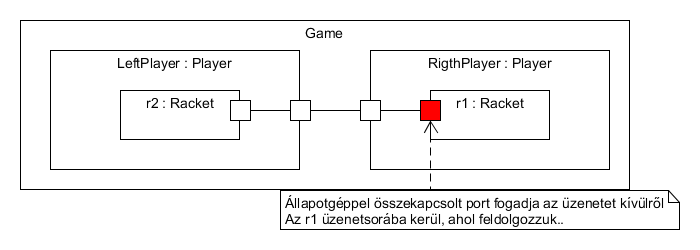
\includegraphics[scale=0.5]{vedes_demo_class_recived.png}
	\end{center}
	\begin{itemize}
	\item Gyerek komponens referencia helyett az állapotgépre kell referenciát birtokolnunk. 
	\item Más viselkedés, más adattagok.
	\end{itemize}
\end{frame}

\begin{frame}
	\frametitle{Gyerek felé továbbítás delegáció esetén}
	\begin{center}
	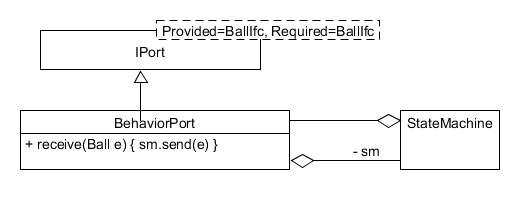
\includegraphics[scale=0.5]{vedes_demo_behav_port.png}
	\end{center}
	\begin{itemize}
	\item A \textit{send} hatására bekerül az állapotgép üzenetsorába az \textit{Ball} üzenet.
	\item Tudnunk kell, melyik portról érkezett az üzenet, amikor átmenetben dolgozzuk fel.
	\end{itemize}
\end{frame}

\begin{frame}
	\frametitle{Gyerek felé továbbítás delegáció esetén}
	\begin{center}
	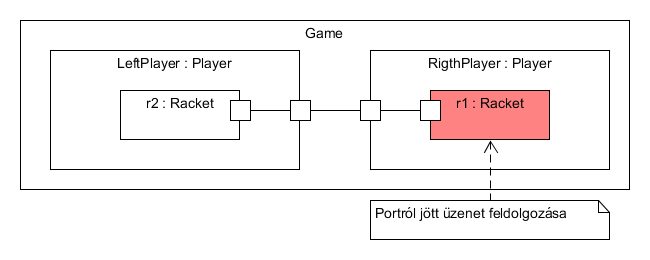
\includegraphics[scale=0.5]{vedes_demo_recived_proc.png}
	\end{center}
	\begin{itemize}
	\item Átmeneteknél (esemény,állapot) mellett megadhatjuk, mely portokról jött üzenetek relevánsak az átmenet szempontjából.
	\item Állapotgép reprezentálása mint eddig, figyelembe véve, honnan érkezett az üzenet (átmenet tábla bővítése, maszkolás). 
	\end{itemize}
\end{frame}

\begin{frame}
	\frametitle{Összefoglalás, eredmények}
	\begin{itemize}
	\item Az UML kompozit szabvány alapos értelmezése, a megfelelő reprezentációk és szemantika megtalálása.
	\item C++ kódgenerálási stratégiák készítése.
	\item Szabványos modell generálása txtUML modell alapján, egy stratégia implementációja.
	\item A diplomamunka összefoglalja, hogy miben segítenek a portok a modellezésben (könnyebb párhuzamosíthatóság, jobb FMU wrapper, példamodellek készítése oktatási célokra komponens-alapú oktatáson, stb.).
	\end{itemize}
\end{frame}

\begin{frame}
	\frametitle{Komponens-alapú UML modellek fordításának vizsgálata}
	\begin{center}
		\Large{Köszönöm a figyelmet!}
	\end{center}
\end{frame}

\end{document}
